\documentclass[aspectratio=169,xcolor=pdftex,dvipsnames]{beamer} % dynamic slides
%\documentclass[[aspectratio=169,handout,xcolor=pdftex,dvipsnames,table]{beamer} % handout

%\usepackage{sslides}
\usepackage{multirow}
\usepackage{verbatim}
\usepackage{amssymb,amsmath}

\usepackage{graphicx}
\usepackage{tikz}

%% to support German characters like äöü 
%\usepackage[]{fontenc}
%\usepackage[latin1]{inputenc} 
%\usepackage[austrian]{babel}

%% graphics
\usepackage{graphicx}
\graphicspath{
    {images/}
}

%%----------------------------------------------------------------
%% comment if fancyheadings.sty is not installed (e.g., for MikTex)
%% you can change the logo in the file fancyheadings.tex
%\input{includes/fancyheadings}

\newcommand{\jname}[1]{\textsf{#1}}

%% most beamers can't project decent colors so I set them to max!
%% redefine emph color
%\definecolor{Emph}{rgb}{1,0,0}  %red
\definecolor{Emph}{rgb}{0.7,0.1,0.1}  %softer red for display
\renewcommand{\emph}[1]{\textcolor{Emph}{\bf\textit{#1}}}

%% define color for slide titles
%\definecolor{Title}{rgb}{0,0,1}  %blue
\definecolor{Title}{rgb}{0.2,0.2,0.6}  %softer blue for display
\definecolor{Gold}{RGB}{255,215,0}
%\definecolor{Title}{rgb}{1,0,0}  %red

\newcommand{\jemph}[1]{\textcolor{Blue}{\textbf{#1}}}

\newcommand{\jconstantname}[1]{\textsf{#1}}
\newcommand{\jDefine}[1]{{\bf #1}}
%\input{../preamble/jgreek.tex}
%\input{../preamble/jsymbols.tex}

% SPACING
\newcommand{\spac}[1]{{\makebox[#1]{}}}
\newcommand{\jblankline}{\ \\ \ \\ }
%\renewcommand{\newpage}{\vfill\pagebreak}
\newcommand{\novspace}{\vspace{-.125in}} %use after description environment.
\newcommand{\centerone}[1]{{{\makebox{\ }}{\hfill #1\hfill}{\makebox{\ }}}}
\newcommand{\centertwo}[2]{{{#1}\hfill{#2}\hfill{\makebox{\ }}}}

% FONTS
\newcommand{\bi}[1]{\mbox{\boldmath $#1$}} % bold italic
\newcommand{\rmitem}[1]{\item[{{\rm #1}}]} % use in: description

%---------------------------------------------------------------------------------------------------

%%%%%%%%%%%%%%%%%%%%%%%%%%%%%%%%%%%%%%%%%%%%

\title{\textbf{Discovering the Mechanics of the Solar System}}
\author{\textbf{\Large Jan Plaza}\\ \ \\
github.com/plazajan}
%\date{SUNY Plattsburgh Totality Conference\\ \ \\ April 6, 2024
%\\ \ \\ \ \\ \ \\
%\tiny{\copyright 2024 Jan Plaza, licensed under CC BY 4.0}
%}

% 60 minute presentation

\begin{document}

%\maketitle

%----------------------------------------------------------------------------------------------------
{
\setbeamertemplate{background}
{
    \includegraphics[width=\paperwidth]{vanGoghStarryNight.jpg}
}
\begin{frame}
\frametitle{\textcolor{white}{\textbf{Two things awe me most:}}}
 
 \textcolor{white}{
{\Huge\textbf{the starry sky above me,\\ \ \\
the moral law within me.}
\ \\ \ \\ \ \\
Immanuel Kant
}}

\end{frame}
}

%----------------------------------------------------------------------------------------------------

\maketitle

%----------------------------------------------------------------------------------------------------

%\begin{frame}
%\frametitle{Plan}
% 
%Discovering the Mechanics of the Solar System 
%- A narrative of the history of humanity's understanding of celestial mechanics, 
% from prehistoric times to Newton: \\ \ \\
%\begin{itemize}
%\item
%Astronomers and discoveries,
%
%\item
%mathematics,
%\item
%physics,
%\item
%computer simulations,
%\item
%methodology of science.
%\end{itemize}
%
%\end{frame}

%----------------------------------------------------------------------------------------------------
{
\setbeamertemplate{background}
{
    \includegraphics[width=\paperwidth]{sunAndMoon.jpg}
}
\begin{frame}
\frametitle{\textcolor{white}{\hspace{7cm}Prehistoric times: Earth, Sun and Moon}}
 
\end{frame}
}

%----------------------------------------------------------------------------------------------------

{
\setbeamertemplate{background}
{
    \includegraphics[width=\paperwidth]{milkyWay.jpg}
}
\begin{frame}
\frametitle{\textcolor{white}{Prehistoric times: stars, Milky Way}}
 
\end{frame}
}

%----------------------------------------------------------------------------------------------------

{
\setbeamertemplate{background}
{
    \includegraphics[width=\paperwidth,height=\paperheight]{comet.jpg}
}
\begin{frame}
\frametitle{\textcolor{white}{Prehistoric times: comets}}
 
\end{frame}
}

%----------------------------------------------------------------------------------------------------
{
\setbeamertemplate{background}
{
    \includegraphics[width=\paperwidth]{solarEclipse.jpg}
}
\begin{frame}
\frametitle{\textcolor{white}{Prehistoric times: solar eclipses\\
First records:\\
772 BCE, China\\
750 BCE, Babylon}}
 
\end{frame}
}

%----------------------------------------------------------------------------------------------------

{
\setbeamertemplate{background}
{
    \includegraphics[width=\paperwidth]{solstice.jpg}
}
\begin{frame}
\frametitle{\textcolor{white}{Prehistoric times:} \textcolor{black}{noon, seasons, solstices, year}}
 
\end{frame}
}


%----------------------------------------------------------------------------------------------------

{
\setbeamertemplate{background}
{
    \includegraphics[width=\paperwidth,height=\paperheight]{wanderingStars.jpeg}
}
\begin{frame}
\frametitle{\textcolor{white}{\hspace{3.5cm}Prehistoric times: wandering stars, ecliptic}}
 
\end{frame}
}

%----------------------------------------------------------------------------------------------------

{
\setbeamertemplate{background}
{
    \includegraphics[width=\paperwidth,height=\paperheight]{ursaMajor.png}
}
\begin{frame}
\frametitle{\textcolor{white}{Prehistoric times:\\ constellations}}
 
\end{frame}
}


%----------------------------------------------------------------------------------------------------

{
\setbeamertemplate{background}
{
    \includegraphics[width=\paperwidth]{starTrails.jpg}
}
\begin{frame}
\frametitle{\textcolor{white}{Prehistoric times: star trails, pole star\\
Phoenicia: navigation by the pole star}}
 
\end{frame}
}




%----------------------------------------------------------------------------------------------------
{
\setbeamertemplate{background}
{
    \includegraphics[width=\paperwidth]{lunarEclipse.jpg}
}
\begin{frame}
\frametitle{\textcolor{white}{Prehistoric times: lunar eclipse.\\ Mesopotamia, 8$^{\text{th}}$ century BCE: 18-year cycle.}}
 
\end{frame}
}

%----------------------------------------------------------------------------------------------------
\begin{frame}
\frametitle{Early civilization, Sumeria and Babylon: angular measures}

\hspace{-1cm}
\includegraphics[width=50mm]{equilateralTriangle.pdf}\  \ \  
\includegraphics[width=60mm]{angularDiameter.jpg}

\begin{itemize}
\item
$1^\circ$ (degree) $\approx$ the pinky at arm's length. 
\item
$1^\circ=60'$ (arc minutes).
\item
$1'=60''$ (arc seconds).
\item
$1'$ (arc second) $\approx$ human eye resolution limit.
\item
Angular diameter of the Moon $\approx 0.5^\circ$.
\item
Angular diameter of the Sun $\approx 0.5^\circ$.
\item
Angular diameters of planets -- too small to measure without telescopes.
\end{itemize}

\end{frame}

%----------------------------------------------------------------------------------------------------
\begin{frame}
\frametitle{Thales of Miletus, 6$^{\text{th}}$ century BCE}

\begin{tikzpicture}[scale=1]
%\draw[line width=0.1pt,gray!30,step=1mm]
%     (0,0) grid (8,5);
%\draw[help lines]
%     (0,0) grid (8,5);
\draw (6,5) -- (0,0) -- (7,3);
\draw[dashed, thick, red](6,5) -- (7,3);
\draw (6.5,4) ellipse[x radius=1.1, y radius=0.3, rotate=115];
\draw[dashed, thick, red](3,2.5) -- (3.5,1.5);
\draw (3.25,2) ellipse[x radius=0.55, y radius=0.15, rotate=115];
%\draw (0,0) -- 
\end{tikzpicture}
 \ \ \ \  \ \ \ \ \ 
\includegraphics[width=35mm]{thales.jpg}

\begin{itemize}
\item
A Greek mathematician and philosopher.
\item
A theorem on similar triangles.
\item
Later used for celestial objects with equal angular measures:\\
the ratio of diameters equals the ratio of distances.
\end{itemize}

\end{frame}


%----------------------------------------------------------------------------------------------------
\begin{frame}
\frametitle{Eratosthenes of Cyrene, 3$^{\text{rd}}$ century BCE}
% c. 276 BCE - c. 194 BCE

\begin{columns}
        
\column{0.35\linewidth}
      \includegraphics[width=55mm]{eratosthenes.png}
\column{0.65\linewidth}
\begin{itemize}
\item
A Greek polymath: mathematician, geographer, poet, astronomer, music theorist,\\
chief librarian at the Library of Alexandria.
\item
The first to calculate Earth's circumference.
\item
Sun's diameter relative to to that of the Earth.
\item
The distance between the Earth and the Sun.
\item
How? By the Thales' theorem!
%\item
%No original works survived the destruction of the Library of Alexandria.
\end{itemize}

\end{columns} 

\end{frame}

%----------------------------------------------------------------------------------------------------
\begin{frame}
\frametitle{Earth's circumference, 3$^{\text{rd}}$ century BCE}

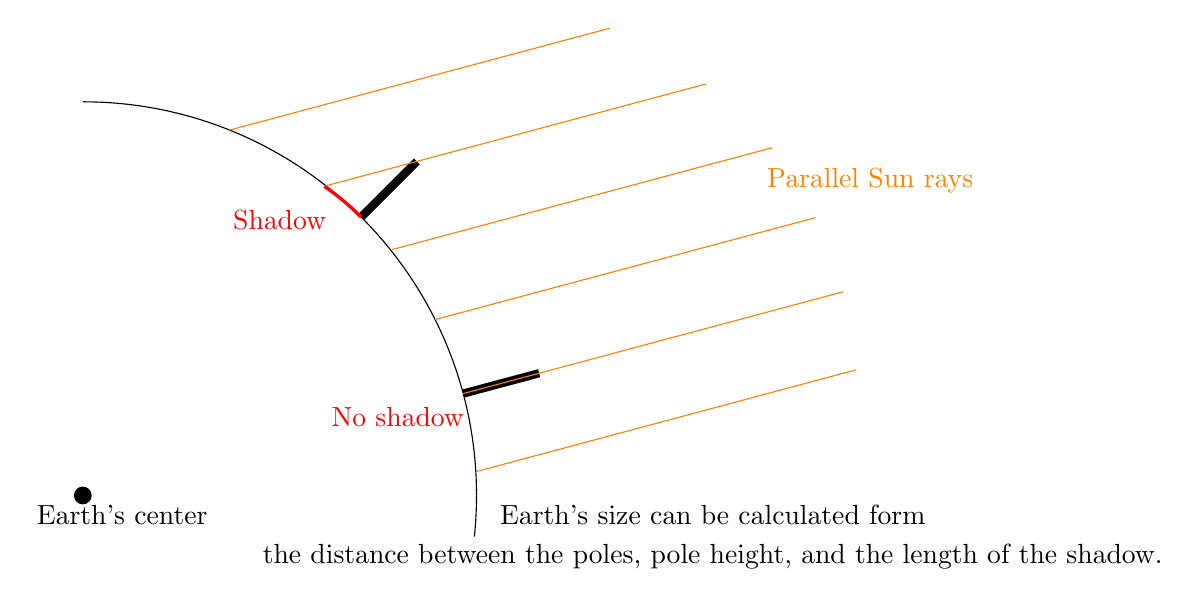
\begin{tikzpicture}[scale=1]

%\draw[line width=0.1pt,gray!30,step=1mm]
%     (0,0) grid (8,6);
%\draw[help lines]
%     (0,0) grid (8,6);

\draw[fill] (0,0) circle[radius=3pt];
\node[below] at (0.5,0) {Earth's center};

\draw (5,0) arc (0:90:5);
\draw (5,0) arc (0:-6:5);
\draw[line width=3pt, rotate=15] (5,0) -- (6,0); % lower pole

\draw[line width=3pt, rotate=45] (5,0) -- (6,0); % upper pole
\draw[red, very thick, rotate=45] (5,0) arc (0:10:3.5); % shadow

\node[red] at (4,1) {No shadow};
\node[red] at (2.5,3.5) {Shadow};

\draw[orange, rotate=15, shift={(-2.0,4)}] (5,0) -- (10,0);
\draw[orange, rotate=15, shift={(-1.0,3)}] (5,0) -- (10,0);
\draw[orange, rotate=15, shift={(-0.4,2)}] (5,0) -- (10,0);
\draw[orange, rotate=15, shift={(-0.1,1)}] (5,0) -- (10,0);
\draw[orange, rotate=15]                           (5,0) -- (10,0);
\draw[orange, rotate=15, shift={(-0.1,-1)}] (5,0) -- (10,0);

\node[orange] at (10,4) {Parallel Sun rays};

\node[below] at (8,0) {Earth's size can be calculated form}; 
\node[below] at (8,-0.5) {the distance between the poles, pole height, and the length of the shadow.};


\end{tikzpicture}

\end{frame}

%----------------------------------------------------------------------------------------------------
\begin{frame}
\frametitle{Aristarchus of Samos, 3$^{\text{rd}}$ century BCE}
%c. 310 BCE - c. 230 BCE


\begin{columns}

\column{0.35\linewidth}
      \includegraphics[width=45mm]{aristarchus.jpeg}
\column{0.65\linewidth}
\vspace{-10mm}

\begin{itemize}
\item
A Greek astronomer and mathematician.

\item
The first known heliocentric model\\
soon forgotten due to the influence of Aristotle.
\item
Sizes and distances of the Earth, Moon and Sun.
\item
How? By observation/measurement of Sun and Moon eclipses, Moon phases, and Thales' theorem.
\end{itemize}

\end{columns} 

\end{frame}

%----------------------------------------------------------------------------------------------------
\begin{frame}

\centering
\pause
\LARGE{
And now, \pause 
we all will conduct\pause
\\
the great experiment of\pause
\\ \ \\
{\Huge{The Thumb Parallax}}\pause
\\ \ \\
which dates back to prehistoric times\pause
\\
or early childhood!
}

\end{frame}

%----------------------------------------------------------------------------------------------------
\begin{frame}
\frametitle{The Thumb Parallax Experiment}

\begin{enumerate}
\item
Outstretch one hand with the thumb up. Hold it still.\\
Close one eye.\\
Observe the relative position of the thumb with respect to the distant background.\\
Switch eyes.\\
Observe the relative position of the thumb with respect to the distant background.\\
Does the thumb seem to move?\\
The angular measure of the movement is called parallax.
\item
Bring the thumb closer, half of the previous distance. Hold it still.\\
Close one eye.\\
Observe the relative position of the thumb with respect to the distant background.\\
Switch eyes.\\
Observe the relative position of the thumb with respect to the distant background.\\
Does the thumb seem to move more or less than in the previous experiment?
\end{enumerate}

The closer the thumb the more it seems to move -- the bigger the parallax!\\ 
From the parallax one can calculate the distance!

\end{frame}



%----------------------------------------------------------------------------------------------------
\begin{frame}
\frametitle{Greece, $3^{\text{rd}}$ century BCE: lunar parallax}

\begin{columns}
        
\column{0.5\linewidth}
      \includegraphics[width=75mm]{lunarParallax.png}
           
\column{0.5\linewidth}
Lunar parallax -- the angle of the apparent shift of the Moon while viewed form different places.\\

Measuring the distance to the Moon:
           \begin{itemize}
           \item
           Aristarchus, Greece, 3$^{\text{rd}}$ century BCE.
           \item
           Hipparchus, Greece, 2$^{\text{nd}}$ century BCE.
           \item
           Ptolemy, Alexandria, 2$^{\text{nd}}$ century CE.
           \item
           Hipparchus and Ptolemy\\ used trigonometry.
           \item
            2007 amateur measurement,\\
             from places 1600 miles apart,\\
            has shown a $0.5'$ shift
             with respect to the 
             background star Regulus;\\ 
             11\% error in the Moon's distance.
            \end{itemize}
\end{columns} 
\ \\
\hspace{-0.7cm}
Current measurement by laser ranging, Moon elliptical orbit's
semi-major axis: 384,399 km

\end{frame}


%----------------------------------------------------------------------------------------------------
\begin{frame}
\frametitle{Hipparchus of Nicea, 2$^{\text{nd}}$ century BCE: trigonometry}
% c. 190 BCE - c. 120 BCE

\centering
\begin{columns}
\column{0.5\linewidth}
\ \ \ \ \ \includegraphics[width=36mm]{hipparchus.jpg}            
\column{0.5\linewidth}
\vspace{4mm} \includegraphics[width=84mm]{earthPrecession.pdf} 
\end{columns} 
 
\begin{itemize}
\item
A Greek mathematician, the founder of trigonometry.
\item
Accurate quantitative model of sizes, distances and motion of the Sun and Moon; and of eclipses.
The Moon and Sun revolve around the Earth.\\
(Notice that mathematically, geocentric $\equiv$ heliocentric, if there are  no planets.)
\item
Precession of Earth's axis (period 26,000 years).
\end{itemize}
 
\end{frame}

%----------------------------------------------------------------------------------------------------
\begin{frame}
\frametitle{Claudius Ptolemy, 2$^{\text{nd}}$ century}

\begin{columns}

\column{0.4\linewidth}
      \includegraphics[width=50mm]{ptolemy.jpg}
\column{0.6\linewidth}
\vspace{-10mm}
\begin{itemize}
\item
An Alexandrian mathematician, astronomer, astrologer, geographer, music theorist
\item
13-volume Almagest\\
- a compendium of ancient astronomy,\\ with astronomical tables spanning 800 years.
\item
Geocentric model of the universe. 
\end{itemize}

\end{columns} 

\end{frame}

%----------------------------------------------------------------------------------------------------

\begin{frame}
\frametitle{Ptolemaic geocentric model}

\begin{columns}
        
\column{0.5\linewidth}
      \includegraphics[width=70mm]{geocentric.pdf}
\column{0.5\linewidth}
           Spherical Earth at the ``center".\\
           Moon, planets, Sun, each
           revolving around separate equant points,\\
           on a small  circle (epicycle)\\
           whose center moves on a big circle (deferent). 
\end{columns} 
\ \\
Later, second-order epicycles were added\\
to improve predictions of positions of planets, and of eclipses.

\end{frame}


%----------------------------------------------------------------------------------------------------

\begin{frame}
\frametitle{Stellar Parallax}

\begin{columns}
        
\column{0.4\linewidth}
      \includegraphics[width=70mm]{parallax.pdf}
\column{0.6\linewidth}
Stellar parallax of a near star --
the angle of apparent shift when viewed from two points\\ on the Earth's (hypothetical?) orbit around the Sun.
\\ \ \\
 The ancients looked for a stellar parallax,\\
 but it was unnoticeable without telescopes\\
 -- the main scientific argument\\
  against the heliocentric system.
 
  \end{columns} 

\end{frame}

%----------------------------------------------------------------------------------------------------

\begin{frame}
\frametitle{Ptolemaic geocentric model dominates for 13 centuries}

\begin{itemize}
\item
Both in Europe and in the Islamic world.
\item 
``If the Earth were moving, we would be blown off its surface.''
\item
``We are the most important\\ -- the Earth must be the center of the universe.''
\item
Pythagoreanism considers mathematics to be the essence of reality,\\
implying mathematical perfection of the universe: \\
perfect circles, revolving ``crystal spheres" creating ``heavenly music";\\
a blurred distinction between mathematics and nature.
\item
Ptolemaic geocentric model, rooted in Aristotle,\\ was supported by religious institutions.
\item
Without telescopes (till the 17$^{\text{th}}$ century), stellar parallax was unnoticeable, leading Tycho Brahe and most thinkers before him to believe Earth does not move.  
\item
Current view: tolerable predictions, but fitting a square peg into a round hole.     
\end{itemize}

\end{frame}

%----------------------------------------------------------------------------------------------------

{
\setbeamertemplate{background}
{
    \includegraphics[width=\paperwidth]{copernicus-matejko.jpg}
}
\begin{frame}
\frametitle{\textcolor{white}{Nicolaus Copernicus, 16$^{\text{th}}$ century}}
 
\end{frame}
}


%----------------------------------------------------------------------------------------------------
\begin{frame}
\frametitle{Nicolaus Copernicus, 1473 - 1543}


\begin{columns}
        
\column{0.3\linewidth}
      \includegraphics[width=50mm]{copernicus.jpg}
\column{0.7\linewidth}
\begin{itemize}
\item
A Polish polymath, mathematical astronomer,\\ medical practitioner,
 church administrator, economist.
\item
Must have studied astrology but did not practice it\\
-- unique in his age.
\item
Formulated quantitative theory of money and Gresham's law in economy.
\item
1532, Heliocentric system\\ (independently of Aristarchus);\\
circular orbits, epicycles but no equants.\\
\item
\textbf{1543}, \textit{De Revolutionibus Orbium Coellestium} published\\
-- the beginning of the Scientific Revolution in Europe.
\end{itemize}
\end{columns} 

\end{frame}


%----------------------------------------------------------------------------------------------------
\begin{frame}
\frametitle{Galileo Galilei, 1564 - 1642}


\begin{columns}
        
\column{0.5\linewidth}
      \includegraphics[width=75mm]{galileo.jpg}
\column{0.5\linewidth}

\begin{itemize}
\item
An Italian astronomer, physicist and engineer.
\item 
Improved the optical telescope.
\item
Experimental and theoretical science, classical physics, applying the scientific method.
\item
The father of modern science.
\item
Confirmed the Copernican heliocentric model through telescope observations:\\
Phases of Venus, moons of Jupyter.
\item
Imprisoned for his work.
\end{itemize}
\end{columns} 

\end{frame}


%----------------------------------------------------------------------------------------------------
\begin{frame}
\frametitle{Tycho Brahe, 1546 - 1601}

\centering
\begin{columns}
       
\column{0.35\linewidth}
\includegraphics[width=55mm]{tychoQuadrant.jpg} 
\column{0.65\linewidth}
\begin{itemize}
\item
A Danish astronomer.
\item
The most advanced and biggest observatory in the pre-telescope era, 
Uraniborg, on the island of Hven.
\item
Very accurate observations of positions of planets by naked eye, over a period of 30 years,
\textbf{c. 1570 - 1601}. $\frac{1}{4}$ of the error of earlier observations.
\item
Chose Johannes Kepler to publish the results;\\
 \textit{Rudolphine Tables}
published by Kepler in \textbf{1627}.
\end{itemize}
   
\end{columns} 

\end{frame}

%----------------------------------------------------------------------------------------------------
\begin{frame}
\frametitle{Tycho Brahe, 1546 - 1601}

\centering
\begin{columns}
\column{0.4\linewidth}
\includegraphics[width=50mm]{sextant.jpg}            
\column{0.6\linewidth}
A colorful persona. Studied in Denmark and Germany. Lost his nose in a duel over math prowess. 
A bronze nose, and a gold-silver one for special occasions.
Astrologer and alchemist. Nobleman, friend of King Frederick II of Denmark. Harsh landlord of peasantry. Angered the new king Christian IV by not maintaining the royal chapel; left Denmark for Prague. Very secretive and stingy. Appointed imperial mathematician by an even more stingy Emperor Rudolf II. Tycho referred to Kepler as ``dear friend", to absolve himself from paying his assistant. Tycho's pet elk died after falling down the stairs while drunk.
\end{columns} 

\end{frame}


%----------------------------------------------------------------------------------------------------
\begin{frame}
\frametitle{Johannes Kepler, 1571 - 1630}

\begin{columns}
        
\column{0.5\linewidth}
      \includegraphics[width=55mm]{kepler.jpg}
\column{0.5\linewidth}
          A German mathematician, astronomer, astrologer, first science fiction writer.
          \\ \ \\
          \includegraphics[width=55mm]{keplerSolarSystem.png}
\end{columns} 

\end{frame}

%----------------------------------------------------------------------------------------------------
\begin{frame}
\frametitle{Ancient Greece: ellipse}

\begin{columns}
\column{0.5\linewidth}

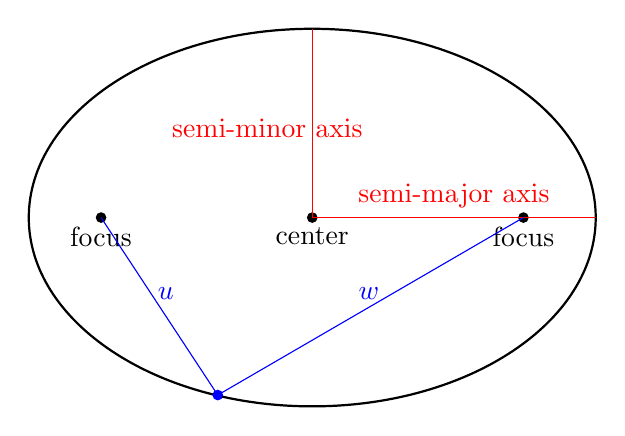
\begin{tikzpicture}[scale=0.6]

%\draw[line width=0.1pt,gray!30,step=1mm] (-6,-4) grid (6,4);
%\draw[help lines] (-6,-4) grid (6,4);

\draw[thick,xscale=1, yscale=0.666] (0,0) circle[radius=6];
\draw[fill] (0, 0) circle[radius=0.1];
\draw[fill] (4.47, 0) circle[radius=0.1];
\draw[fill] (-4.47, 0) circle[radius=0.1];
\node[below] at (0,0) {center};
\node[below] at (4.47,0) {focus};
\node[below] at (-4.47,0) {focus};

\draw[red] (0,0) -- (0,4);
\node[red] at (-0.95,1.9) {semi-minor axis};
\draw[red] (0,0) -- (6,0);
\node[red] at (3,0.45) {semi-major axis};

\draw[fill,blue] (-4.47,0) -- (-2,-3.757) circle[radius=0.1] -- (4.47,0);
\node[blue] at (-3.1,-1.6) {$u$};
\node[blue] at (1.2,-1.6) {$w$};


\end{tikzpicture}

\column{0.5\linewidth}
\begin{itemize}
\item
Draw a circle on a rubber sheet,\\
and stretch it horizontally\\
-- you get an ellipse.
\item
Draw a circle\\
 on a vertically stretched rubber sheet,\\
and let it shrink\\
 -- you get an ellipse.
\item
\textcolor{blue}{$u+w=\text{constant}$}
 \item
 When the foci coincide,\\ the ellipse is a circle.
\end{itemize}

\end{columns} 

\end{frame}
%----------------------------------------------------------------------------------------------------
\begin{frame}
\frametitle{Kepler's laws, 1609 - 1619}

\begin{columns}
\column{0.5\linewidth}

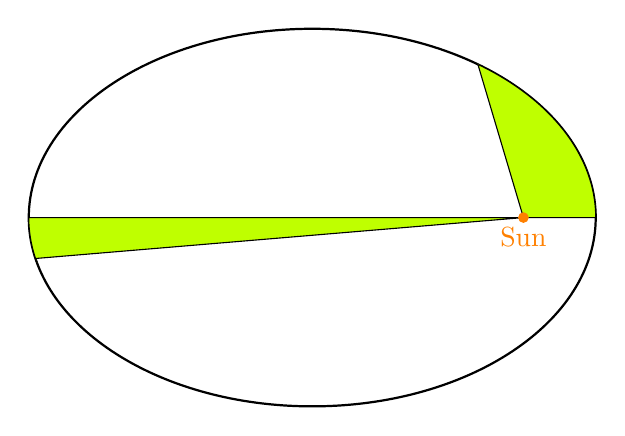
\begin{tikzpicture}[scale=0.6]

%\draw[line width=0.1pt,gray!30,step=1mm] (-6,-4) grid (6,4);
%\draw[help lines] (-6,-4) grid (6,4);

\draw[thick, xscale=1, yscale=0.666] (0,0) circle[radius=6];

\filldraw[fill=lime, xscale=1, yscale=0.666]  (3.5, 4.9) -- (4.47, 0) -- (6, 0) 
                  arc[start angle=0, end angle=54, radius=6];
                  
\filldraw[fill=lime, xscale=1, yscale=0.666]  (-5.85, -1.3) -- (4.47, 0) -- (-6, 0) 
                  arc[start angle=180, end angle=195, radius=6];

\draw[orange,fill] (4.47, 0) circle[radius=0.1];
\node[orange,below] at (4.47,0) {Sun};

\end{tikzpicture}

\column{0.5\linewidth}

Empirical laws of planetary motion\\
(based on Tycho's observations):
\\ \ \\
\begin{enumerate}
\item 
The orbit of a planet is an ellipse\\ with the Sun in a focus.
\item
The line joining a planet and the Sun\\
 sweeps out equal areas\\ during equal intervals of time.\\
(Based on observations of Mars.)
\item 
The square of the orbital period\\ is proportional to\\ the cube of the semi-major axis.
\end{enumerate}

\end{columns} 

\end{frame}

%----------------------------------------------------------------------------------------------------
%\begin{frame}
%\frametitle{}
%
%$a,\ b$ -- semi-major axis, semi-minor axis,\\
%$c$ -- linear eccentricity = focus-to-center distance,\\
%$A,\ P$ -- aphelion, perihelion.
%\\ \ \\
%\textbf{Calculating from $a,\ b$.}\\
%$2c + 2(a-c) = 2\sqrt{b^2+c^2}$\\
%So,\\
%$a^2 = b^2+c^2$\\
%$c = \sqrt{a^2-b^2}$\\
%$P=a-c$\\
%$A=a+c$\\
%\ \\
%\textbf{Calculating from $A,\ P$.}\\
%$a=\frac{1}{2}(A+P)$,\\
%$c=a-P = \frac{1}{2}(A-P)$,\\
%$b^2= a^2-c^2 = AP$,\\
%$b = \sqrt{AP}$.\\
%
%\end{frame}

%----------------------------------------------------------------------------------------------------
%\begin{frame}
%
%\includegraphics[width=90mm]{ellipseParameters2.pdf}\ \\
%
%Eccentricity: $e = \frac{c}{a}= \sqrt{1-\frac{b^2}{a^2}}$, \ \ \ for ellipses, $0< e< 1$,\\
%Linear eccentricity: $c = ae = \sqrt{a^2-b^2}$,\\
%Focal parameter (focus-to-directrix distance): $p = \frac{a}{e}-c$,\\
%Semi-latus rectum: $\ell= pe=\frac{b^2}{a}= \frac{b^2}{\sqrt{a^2-b^2}}$.\\
%
%\end{frame}

%----------------------------------------------------------------------------------------------------
\begin{frame}
\frametitle{Sir Isaac Newton, 1642 - 1727}

\begin{columns}
\column{0.42\linewidth}
      \includegraphics[width=65mm]{newton.jpg}
\column{0.58\linewidth}
          
\begin{itemize}
\item
An English natural philosopher: mathematician, physicist, astronomer, alchemist, theologian.
\item
Classical mechanics.
\item
Optics, theory of color.
\item 
Built the first practical reflective telescope.
\item
Master of the Royal Mint.
\item
President of the Royal Society.
\item
\textbf{1687}, \textit{Principia Mathematica}\\
can be viewed as the start of\\ the Age of Enlightenment.
\end{itemize}

\end{columns} 

\end{frame}

%----------------------------------------------------------------------------------------------------
\begin{frame}
\frametitle{Newton, Philosophiae Naturalis Principia Mathematica: 1687}

\begin{columns}
\column{0.55\linewidth}
      \includegraphics[width=80mm]{divineGeometer.jpg}
\column{0.45\linewidth}
   

\begin{itemize}
\item
Calculus (independently of Leibniz).
\item 
Newton's Laws of Motion:
   \begin{enumerate}
   \item
   A body not subject to forces,\\ is at rest or moves straight\\ at a constant speed.
   \item
   $F = ma$
  \item
  To every action, there is\\ an opposed and equal reaction.
   \end{enumerate}
\item
Law of gravity:
$F = G\frac{M m}{r^2}$
\item 
Newtonian mechanics.
\item
Mathematical derivation\\ of Kepler's Laws.
\end{itemize}
\end{columns} 

\end{frame}


%----------------------------------------------------------------------------------------------------
\begin{frame}
\frametitle{Henry Cavendish, 1731 - 1810}

\begin{columns}
\column{0.5\linewidth}
          \includegraphics[width=60mm]{cavendish.jpg}
\column{0.5\linewidth}
      \textbf{1798}, experimental measurement\\ of the gravitational constant $G$.\\
      Equivalently - of the mass of the Earth.

\includegraphics[width=45mm]{cavendishExperiment.pdf}\ \
\ \\ Current measurement: 
$ G = 6.67430 \cdot 10^{-11}\  \ \text{m}^3 / (\text{kg} \cdot \text{s}^2)$
\end{columns} 




\end{frame}

%----------------------------------------------------------------------------------------------------
\begin{frame}
\frametitle{Enhancements to Kepler's laws}

\textbf{Kepler's 2$^{\text{nd}}$ law}, enhanced, vis viva equation:

$$v^2 = G(M+m) \left(\frac{2}{r} - \frac{1}{a}\right)$$

\textbf{Kepler's 3$^{\text{rd}}$ law}, enhanced:

$$ \frac{T^2}{a^3} = \frac{4\pi^2}{G(M+m)}$$

where:\\
$T$ -- orbital period,\\
$a$ -- semi-major axis,\\
$G$ -- gravitational constant,\\
$M,\ m$ -- masses,\\
$v$ -- speed,\\
$r$ -- radius i.e. distance $M$ to $m$.
%$\mu = G(M+m)$ -- gravitational parameter.

\end{frame}

%----------------------------------------------------------------------------------------------------
\begin{frame}
\frametitle{Weighing the Sun and planets with moons}

\textbf{Kepler's 3$^{\text{rd}}$ law under the assumption that $M \gg m$ : }
$$ \frac{T^2}{a^3} \approx \frac{4\pi^2}{GM} \ \ \ \ \Rightarrow \ \ \ \  M\approx\frac{4\pi^2}{G}\cdot \frac{a^3}{T^2}$$
\noindent
The orbital period $T$ and semi-major axis \ $a$  \ are observable.\\
The mass $M$ is not observable, but it can be calculated from this equation!
$$ M_\text{sun}\approx\frac{4\pi^2}{G}\cdot \frac{a_\text{earth}^3}{T_\text{earth}^2} \approx 1.9885\cdot 10^{30} \text{kg} $$
$$\  \  \ M_\text{mars}\approx\frac{4\pi^2}{G}\cdot \frac{a_\text{phobos}^3}{T_\text{phobos}^2} \approx 6.4171\cdot 10^{23} \text{kg} $$
$$ M_\text{jupiter}\approx\frac{4\pi^2}{G}\cdot \frac{a_\text{io}^3}{T_\text{io}^2} \approx 1.8982 \cdot 10^{27} \text{kg} $$
\end{frame}

%----------------------------------------------------------------------------------------------------
\begin{frame}
\frametitle{Kepler's world - a computer simulation}



\begin{columns}
\column{0.45\linewidth}
      \includegraphics[width=70mm]{keplersWorld.png}
\column{0.55\linewidth}
   

\begin{itemize}
\item
A computer simulation of orbits resulting from the continuing local effect of the Newton's law of gravity $F = G\frac{M m}{r^2}$
\item
Tests if the simulated planets obey (global) Kepler's laws 1 and 3.
\item 
The screenshot on the left:\\ \textcolor{darkgray}{Mercury}, \textcolor{YellowOrange}{Venus}, 
\textcolor{blue}{Earth}, \textcolor{red}{Mars}.
\item
Verified ellipses with the Sun in one focus.
\item
Orbital periods in days,\\ simulation vs. actual:\\
\textcolor{darkgray}{Mercury: 88.77 vs. .87.97 (0.91\% error)}\\
\textcolor{YellowOrange}{Venus: 225.46 vs. 224.7 (0.34\% error)}\\
\textcolor{blue}{Earth: 365.97 vs 365.26 (0.2\% error)}\\
\textcolor{red}{Mars: 687.85 vs 686.98 (0.13\% error)}
\item
Available at \texttt{github.com/plazajan}
\end{itemize}
\end{columns} 

\end{frame}



%----------------------------------------------------------------------------------------------------
\begin{frame}
%\frametitle{Solar System}
%\ \\
\includegraphics[scale=0.305]{planetsSize.jpg}
\\

\includegraphics[scale=0.3126]{planetsDistance.pdf}


\end{frame}

%----------------------------------------------------------------------------------------------------
\begin{frame}
\frametitle{Other discoveries}

Recall: the ecliptic is the plane of Earth's orbit around the Sun.
\begin{itemize}
\item
Orbital planes of the planets are close to,\\ but not identical with the ecliptic.
\item
Moon's orbit is close to, but not in the ecliptic\\ -- so eclipses are rare.
\item
There is an asteroid belt between Mars and Jupyter.\\ Asteroids are not spherical.
\item
Comets are lumps of ice and dust, a few km across,\\ on highly eccentric orbits, with orbital periods of the order of 100 years.
\item
Kuiper belt -- icy objects past Neptune.
\end{itemize}
\ \\ \ \\
The Sun and the Solar System are still evolving\\
 -- fascinating, but not in the scope of this talk.

\end{frame}

%----------------------------------------------------------------------------------------------------
\begin{frame}
\frametitle{Methodology of science}

\begin{itemize}
\item
Abstraction.
\item
Measurements: relative vs. absolute.
\item
Statements: qualitative vs. quantitative.
\item
Approximation (and estimation of error.)
\item
Continuous vs. discrete.
\item
Models: local  vs. global.
\item
Areas of science:
  \begin{itemize}
  \item
  experimental,
  \item
  theoretical,
  \item
  computational.
  \end{itemize}
  \item
The scientific method:\\ 
observe/experiment, construct a model, make predictions, test, repeat.
%(Ironically, Francis Bacon rejected Copernicus' ideas.)
\item
Ockham's razor - given two models with the same predictions, choose the simpler one.
\end{itemize}

\end{frame}

%----------------------------------------------------------------------------------------------------
\begin{frame}

\pause
\Huge{
This is the end \pause 
of Chapter I\pause
\\
of the great book of science.\pause
\\ \ \\
There is more ...\pause
\\ \ \\
Stay curious!
}


\end{frame}

%----------------------------------------------------------------------------------------------------
\begin{frame}
\frametitle{Image credits}

\tiny{

\textbf{Moon at sunset} https://www.wallpaperbetter.com/nature-and-landscape-wallpaper/atmosphere-moon-stars-sunset-hd-87065

\textbf{Milky Way} by ESO/Y. Beletsky - https://web.archive.org/web/20081121184421/http://www.eso.org/gallery/v/ESOPIA/Paranal/phot-33a-07.tif.html, CC BY 4.0, https://commons.wikimedia.org/w/index.php?curid=7398904

\textbf{Star Trails} by A. Duro/ESO - http://www.eso.org/public/potw1631a/

\textbf{Wandering stars} Museum Victoria/Stellarium, CC BY-SA.

\textbf{Ursa Major} by Sanu N - own work, CC BY-SA 4.0, https://commons.wikimedia.org/w/index.php?curid=129448415

\textbf{Soltice/solargraph} by ESO/R. Fosbury/T. Trygg/D. Rabanus - http://www.eso.org/public/potw1039a/, CC BY 4.0, https://commons.wikimedia.org/w/index.php?curid=11610432

\textbf{Comet} by Soerfm - own work, CC BY-SA 3.0, https://commons.wikimedia.org/w/index.php?curid=27495386

\textbf{Lunar eclipse} by Sergei Mutovkin from Irvine, California, United States - Full Eclipse of the Moon as seen in from Irvine, CA, USA, CC BY 2.0, https://commons.wikimedia.org/w/index.php?curid=118047426

\textbf{Paralax} by Srain at English Wikipedia - This image is an altered version of :Image:Stellarparallax2.svg, which is an SVG version of :Image:Stellarparallax2.png. Stellarparallax2.svg was released into the public domain by its creator, Booyabazooka., Public Domain, https://commons.wikimedia.org/w/index.php?curid=4196613

\textbf{Angular diameter of the sun} by Sriram.aeropsn - Own work, Public Domain, https://commons.wikimedia.org/w/index.php?curid=5745197

\textbf{Lunar parallax} Public Domain, https://commons.wikimedia.org/w/index.php?curid=357712

\textbf{Thales} by Wilhelm Meyer - own scan, Public Domain, https://commons.wikimedia.org/w/index.php?curid=11037570

\textbf{Hipparchos} by William Henry Smyth - George F. Chambers, A Handbook of Descriptive and Practical Astronomy, Vol. 3 (4th ed.) https://archive.org/details/handbookofdescri0003geor/page/n10/mode/1up, Public Domain, https://commons.wikimedia.org/w/index.php?curid=134619278

\textbf{Cavendish experiment} diagram by Chris Burks, Chetvorno - own work, public domain.

\textbf{Solar eclipse} by Beccus at English Wikipedia - Transferred from en.wikipedia to Commons by Mike Peel using CommonsHelper., Public Domain, https://commons.wikimedia.org/w/index.php?curid=4528723

}

\end{frame}

%----------------------------------------------------------------------------------------------------

\begin{frame}
\frametitle{Image credits, continued}

\tiny{

\textbf{Tycho's quadrant} by Unknown author - Engraving from the book: Tycho Brahe (1598), Astronomiae instauratae mechanica, Wandsbeck. Downloaded from the online exhibition at the Royal Library; stitching by Axel Boldt, Public Domain, https://commons.wikimedia.org/w/index.php?curid=19389032

\textbf{Sextant} Public Domain, https://commons.wikimedia.org/w/index.php?curid=89871

\textbf{Kepler} by August Köhler - Kepler-Museum in Weil der Stadt, Public Domain, https://commons.wikimedia.org/w/index.php?curid=9406242

\textbf{Platonic solid model} by Johannes Kepler - Johannes Kepler: Mysterium Cosmographicum, Tübingen 1596, Tabula III: Orbium planetarum dimensiones, et distantias per quinque regularia corpora geometrica exhibens., Public Domain, https://commons.wikimedia.org/w/index.php?curid=37300

\textbf{Galileo} by Giuseppe Bertini - Embedding web page: http://www.gabrielevanin.it/S.\%20Marco\%201609.htmImage: http://www.gabrielevanin.it/Bertini.jpg, Public Domain, https://commons.wikimedia.org/w/index.php?curid=9500742

\textbf{Newton} by Godfrey Kneller - File:Portrait of Sir Isaac Newton, 1689.jpg from https://exhibitions.lib.cam.ac.uk/linesofthought/artifacts, Public Domain, https://commons.wikimedia.org/w/index.php?curid=132521185

\textbf{Divine geometer} by William Blake - The William Blake Archive, Public Domain, https://commons.wikimedia.org/w/index.php?curid=106372088

\textbf{Aristarchus} by Dr. Manuel - Own work, Public Domain, https://commons.wikimedia.org/w/index.php?curid=19032134

\textbf{Ptolemy} by Wikimedia Commons, Public Domain, https://commons.wikimedia.org/w/index.php?curid=16043714

\textbf{Epicycles} https://commons.wikimedia.org/w/index.php?curid=486480

\textbf{Planets size} by CactiStaccingCrane - Own work, CC BY-SA 4.0, https://commons.wikimedia.org/w/index.php?curid=117066567

\textbf{Planets distance} By CactiStaccingCrane - Own work, CC0, https://commons.wikimedia.org/w/index.php?curid=124010369

\textbf{Cavendish} By George Wilson - Frontispiece of The Life of the Hon. Henry Cavendish, Public Domain, https://commons.wikimedia.org/w/index.php?curid=7373371

\textbf{Eratosthenes} by Unknown - Transparent background version of File:Eratosthene.01.png, Public Domain, https://commons.wikimedia.org/w/index.php?curid=117929071

\textbf{Copernicus} by Unknown author - http://www.frombork.art.pl/Ang10.htmhttps://www.welt.de/img/kultur/mobile152954235/1212503297-ci102l-w1024/Kopernikus-Gemaelde-in-Krakau.jpg, Public Domain, https://commons.wikimedia.org/w/index.php?curid=113500

\textbf{Copernicus} by Jan Matejko - www.pinakoteka.zascianek.plmuzea.malopolska.pl, Domena publiczna, https://commons.wikimedia.org/w/index.php?curid=18622
}

\end{frame}

%----------------------------------------------------------------------------------------------------
{
\setbeamertemplate{background}
{
    \includegraphics[width=\paperwidth]{vanGoghStarryNight.jpg}
}
\begin{frame}
\frametitle{\textcolor{white}{\textbf{Two things awe me most:}}}
 
 \textcolor{white}{
{\Huge\textbf{the starry sky above me,\\ \ \\
the moral law within me.}
\ \\ \ \\ \ \\
Immanuel Kant
}}

\end{frame}
}


%%%%%%%%%%%%%%%%%%%%%%%%%%%%%%%%%%%%%%%%%%%%

\end{document}

%%%%%%%%%%%%%%%%%%%%%%%%%%%%%%%%%%%%%%%%%%%%
%%%%%%%%%%%%%%%%%%%%%%%%%%%%%%%%%%%%%%%%%%%%
